\begin{figure}[t]
\uwsinglespace
\begin{center}
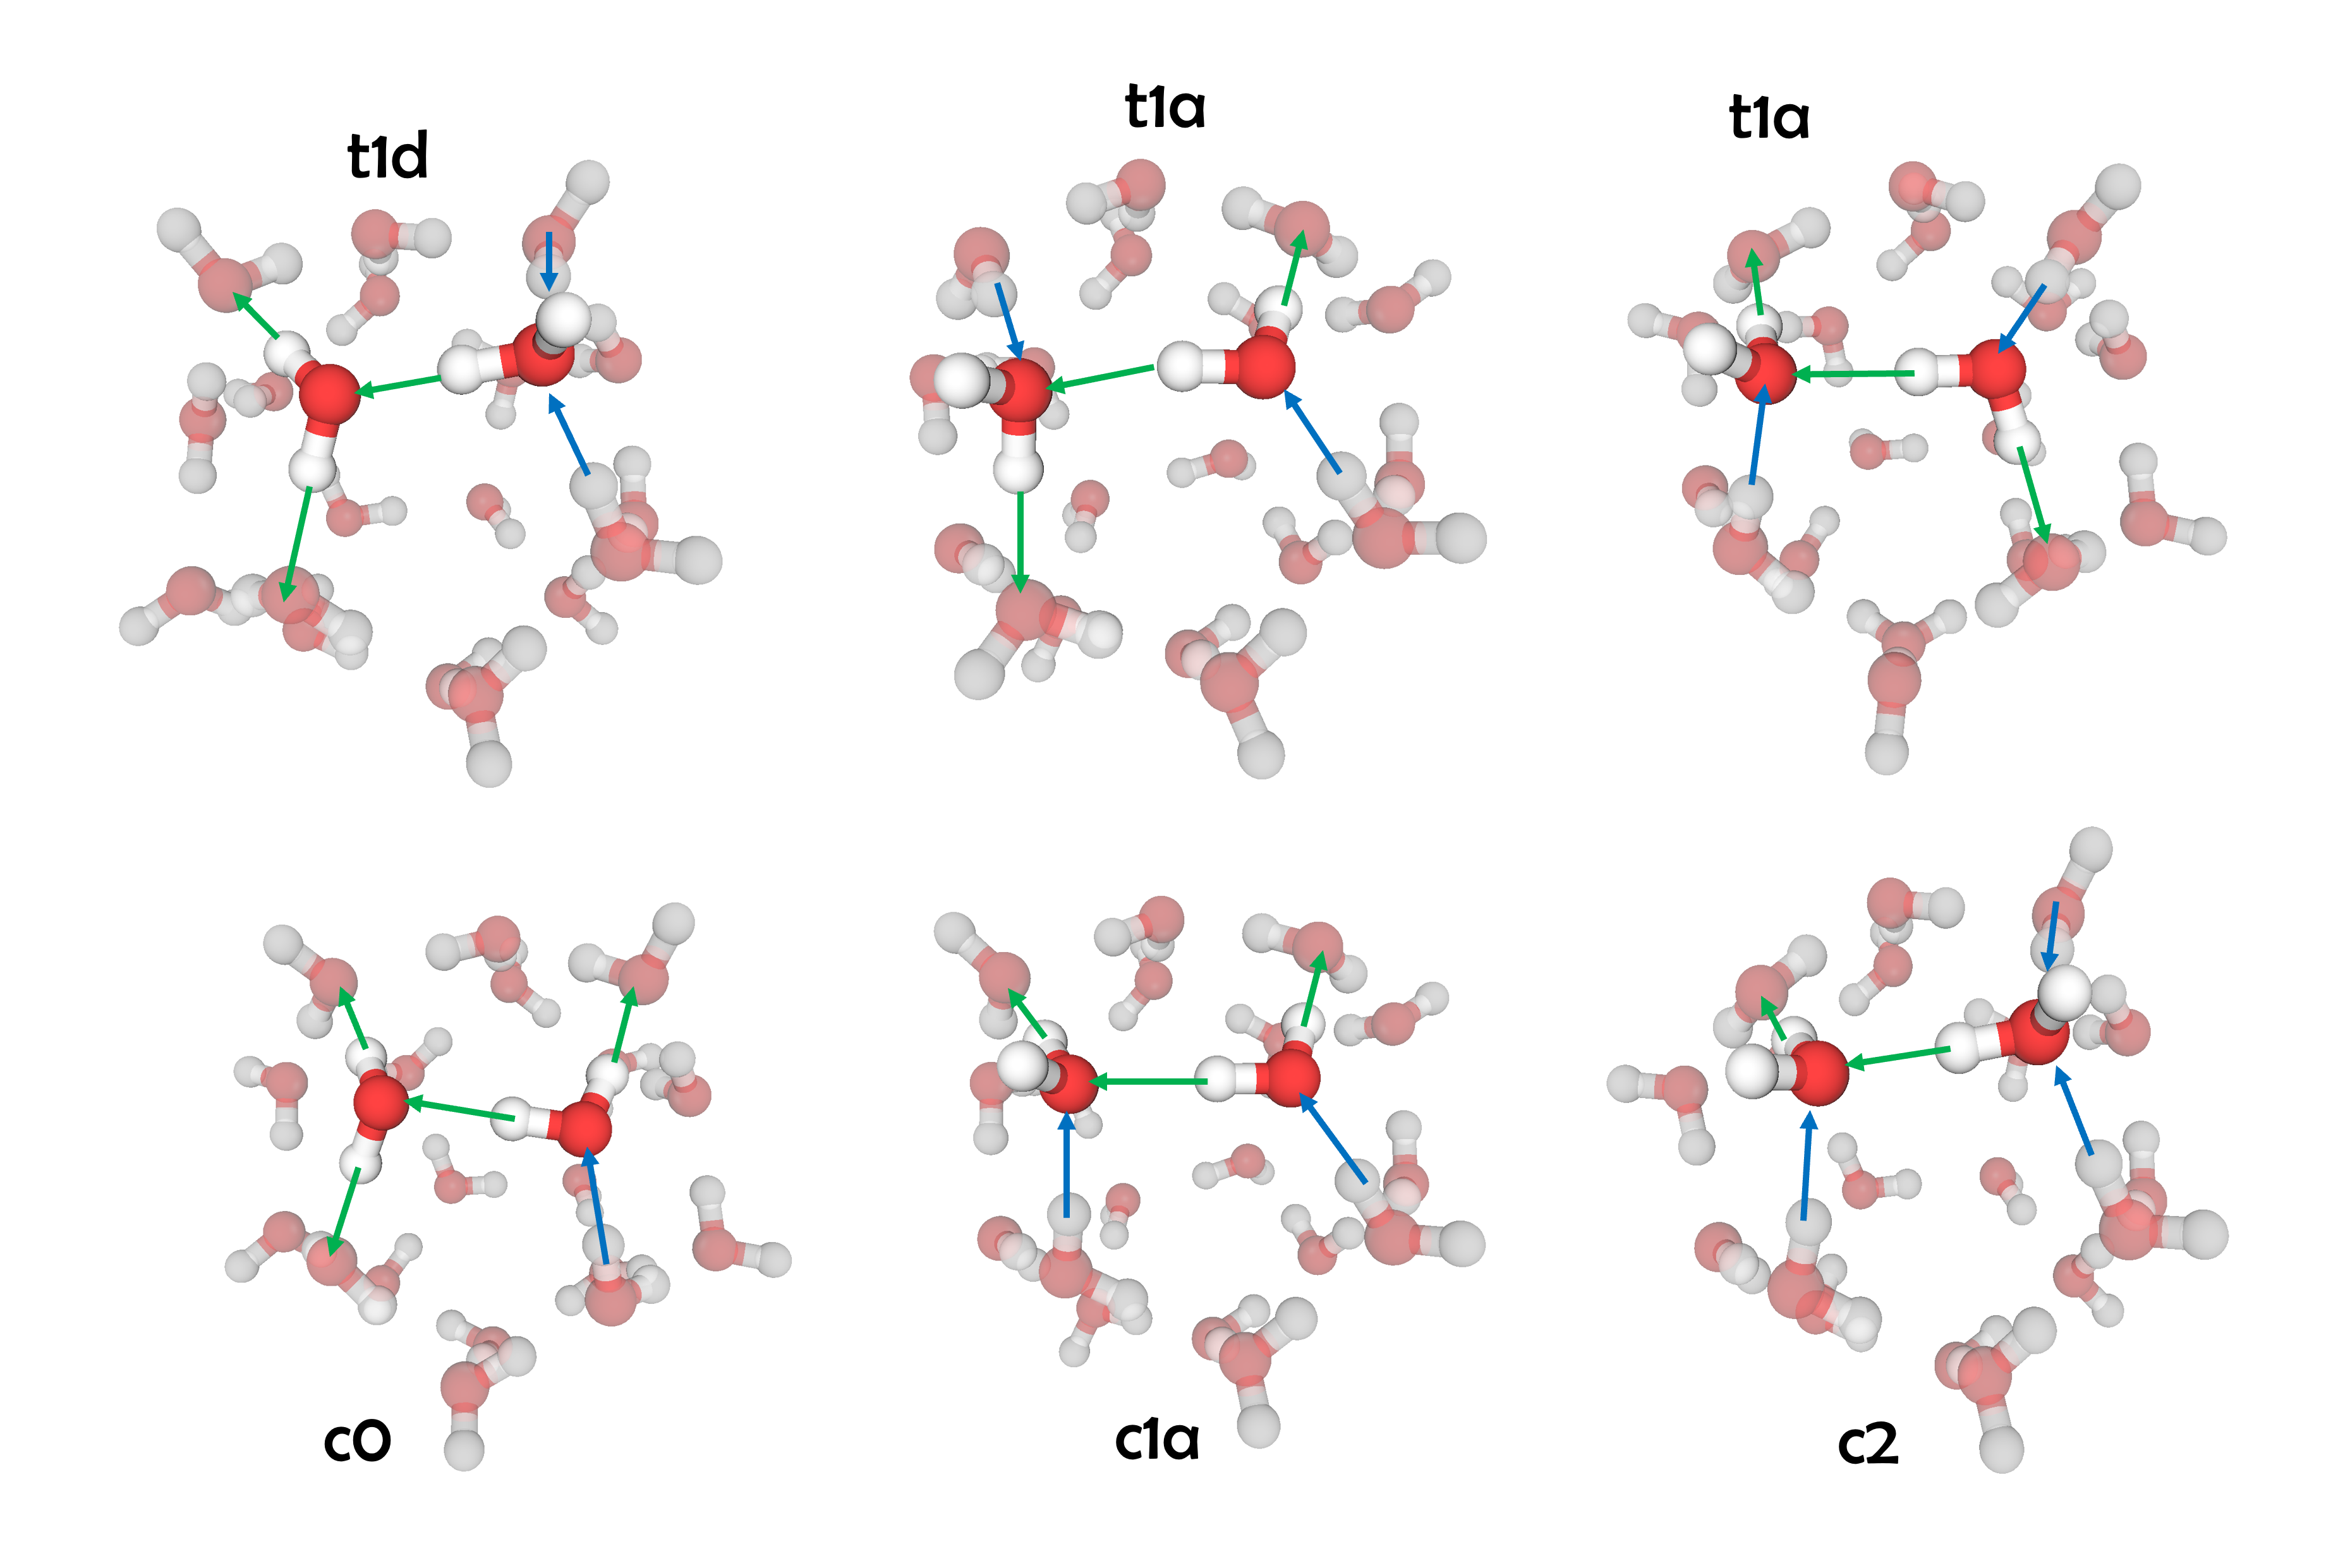
\includegraphics[width=\textwidth]{Figures/Chapter_6/sweb_types.png}
\end{center}
\begin{spacing}{1.0}
\caption[Classification of hydrogen bonds depending on the dimer orientation on the polyhedral surface. Symbols denote trans (t) or cis (c) arrangements and number of hydrogen bonds on either the donor (d) or the acceptor (a) molecules. In the above notation t1d denotes a trans orientation with 1 free OH bond on the hydrogen bond donor molecule. The D-, T- and H-cages have a maximum of 7, 9 and 11 t1d dimers.]{Classification of hydrogen bonds depending on the dimer orientation on the polyhedral surface. Symbols denote trans (t) or cis (c) arrangements and number of hydrogen bonds on either the donor (d) or the acceptor (a) molecules. In the above notation t1d denotes a trans orientation with 1 free OH bond on the hydrogen bond donor molecule. The D-, T- and H-cages have a maximum of 7, 9 and 11 t1d dimers.}\label{fig:MBE_III_F2}
\end{spacing}
\end{figure}